\documentclass[pdftex,12pt,a4paper]{report}
\usepackage[pdftex]{graphicx}
\usepackage{hyperref,pdfpages}
\usepackage[english]{babel}
\usepackage[left=2cm,top=1cm,right=3cm,nohead]{geometry}

\newcommand{\HRule}{\rule{\linewidth}{0.5mm}}

\begin{document}



\begin{titlepage}
\begin{center}

\textsc{\LARGE [CSC318H1]}\\[0.5cm]
\textsc{The Design of Interactive Computational Media}\\[1cm]

\textsc{\Large TA: Christina Christodoulaki}\\[0.5cm]

% Title
\HRule \\[0.4cm]
{ \huge \bfseries Haptic5 Evaluation Report}\\[0.4cm]

\HRule \\[1.5cm]

% Author and supervisor
\begin{minipage}{0.4\textwidth}
\begin{flushleft} \large
\emph{Haptic5 Members:}\\
Taylor\textsc{ Dickson}\\
Victoria\textsc{ Enalen}\\
Wilson\textsc{ Sun}\\
Zhi\textsc{ Zhang}\\
Lia\textsc{ Zheng}\\
\end{flushleft}
\end{minipage}
\begin{minipage}{0.4\textwidth}
\begin{flushright} \large
\emph{Emails:} \\
 me@taylordickson.ca\\
 enalenv@gmail.com \\
 wilson.sun@hotmail.ca\\
 cakyo@live.ca‎\\
 citrus.smooth@gmail.com\\
 
\end{flushright}
\end{minipage}

\vfill

% Bottom of the page
{\large \today}

\end{center}
\end{titlepage}
\tableofcontents

\chapter{Heuristic Evaluation}
A heuristic evaluation was carried out during the February 26th CSC318 tutorial in order to assess conformity of our application to the 5 usability heuristics we have identified as important. This evaluation employed 5 expert evaluators who were asked to complete 2 pre-determined task on paper prototypes and provide feedback based on the 5 heuristics.

\section{Rationale}
Our rationale for using a heuristic evaluation is that the feedback provided by these expert evaluators would yield a greater benefit with a small number of participants leading to decreased time spent. \footnote{As seen on slide 34 in Lecture 6: Usability Principles \& Heuristic Evaluations}

\section{Participants}
We recruited 5 expert evaluators from our CSC318 course at the University of Toronto. These evaluators are male between the ages of 20 to 25. Four of the evaluators are on their way to completing a Computer Science major/specialist, one did not disclose his information. It is important to note that all evaluators are comfortable using a smartphone, as they all own a smartphone, with 2 of the 5 evaluators running iOS on their smartphone, and the rest running an android operating system. These expert evaluators are also quite familiar with heuristic evaluations and are comfortable with the 5 usability heuristics that were explained to them at the start of the usability task.

\section{Usability Criteria}

To carry out the heuristic evaluation we first presented the evaluators with a description of the 5 usability criteria and how they would be important to our application. These criteria are as follows:
\vspace{0.7cm}

\noindent\textbf{[Consistency and Standards]}
\vspace{0.2cm}
\\The icons and actions that are available must be consistent with what the user thinks
the resulting action should be. The icons and actions should also have uniform
meaning throughout the use of the application and relate to the current platform
so as not to confuse the user and to make available actions recognizable.
\pagebreak
\\\textbf{[Flexibility and Efficiency]}
\vspace{0.3cm}
\\The application must have the ability to customize interaction in order to conform
to the current user. Implementation of this is important in order to have quick user
response times and to accommodate all types of users.
\vspace{0.7cm}
\\\textbf{[Error Prevention]}
\vspace{0.3cm}
\\With a restricted set of actions and the ability to edit data, we can ensure that
the user is never confronted with any form of error. While the data input is up to
the users themselves, the app should always provide means of editing data and to
limit choices, for example with the use of radio buttons. Keeping the data collection
methods consistent prevents the application from raising any form of error.
\vspace{0.7cm}
\\\textbf{[Visibility of System Status]}
\vspace{0.3cm}
\\The user should always know of the current status of the application and what
actions are available at that time. Properly titled pages along with current system
readiness, such as an hourglass to indicate that the system is working or busy, will
let the user know what is happening at that very moment.
\vspace{0.7cm}
\\\textbf{[Aesthetic and Minimal Design]}
\vspace{0.3cm}
\\Eliminating unnecessary actions and icons can reveal what the user is able to do at
that moment in time. Since the interface will have a reduced number of actions, it is
relatively easy to keep the screen visually pleasing and at the same time informative,
letting the user know that the only available actions are the ones seen on the screen.

\section{Tasks}
The evaluators were then asked to complete 2 tasks on the paper prototypes. The evaluators were presented with the home screen at the start of each task, and simulation of the task occurred via the evaluator's interaction with the "buttons" on the protoype. Tapping on the keyboard button allows the evaluator to simulate typing on the screen, and tapping on action buttons would present the evaluator with another screen prototype. \footnote{The screen prototypes can be found in the Appendix} The tasks given are as follows:
\vspace{0.7cm}
\\\textbf{Task 1:} Log into the application, get to the log entry screen and complete an entry.
This is performed by tapping on application icon shown in \textit{Screen 1}, inputting a password
if necessary (the details for the password are already given) or choosing a user that does
not have a password (seen in \textit{Screen 4}) and by clicking Add New shown in \textit{Screen 5}. From here it brings the user to the entry screen as seen on \textit{Screen 6} where the user can input data and confirm their entry by clicking OK as seen on \textit{Screen 7}.
\vspace{0.7cm}
\\\textbf{Task 2:} Create a custom category to add to the log entry screen. From the home screen
\textit{Screen 5}, the user should click the Settings icon on the top right-hand corner which will
bring them to \textit{Screen 10}. Users should then click Change Log (bringing them to \textit{Screen 12}) and then click Create New.

\chapter{Cognitive Evaluation}
\section{Rationale}
\section{Tasks}
\section{Participants}

\chapter{Think-aloud Evaluation}
A think aloud is a very straightforward process that requires only a participant and the paper prototype for the application. It involves the participant executing a given task while giving verbal feedback of all actions and thoughts encountered. For a think aloud, speech throughout the entire task is encouraged and needed to gather accurate, user-perspective data. In order for the participants to be comfortable with verbalizing their actions and their thoughts, we provide a few practice sessions involving objects not related to the application in order for them to get used to speaking their actions.

To ensure an accurate presentation of the think aloud for each participant, we have generated a script that will be presented to each participant. The script consists of a basic description that is given to all participants along with practice tasks that can be given until the participant is comfortable with thinking out loud. The practice sessions use a basic calculator since it is an object that most people are familiar with. The familiarity will help users be confident of their actions and pick up the task more readily. The think aloud itself will only require the paper prototype.

\section{Think Aloud Script}
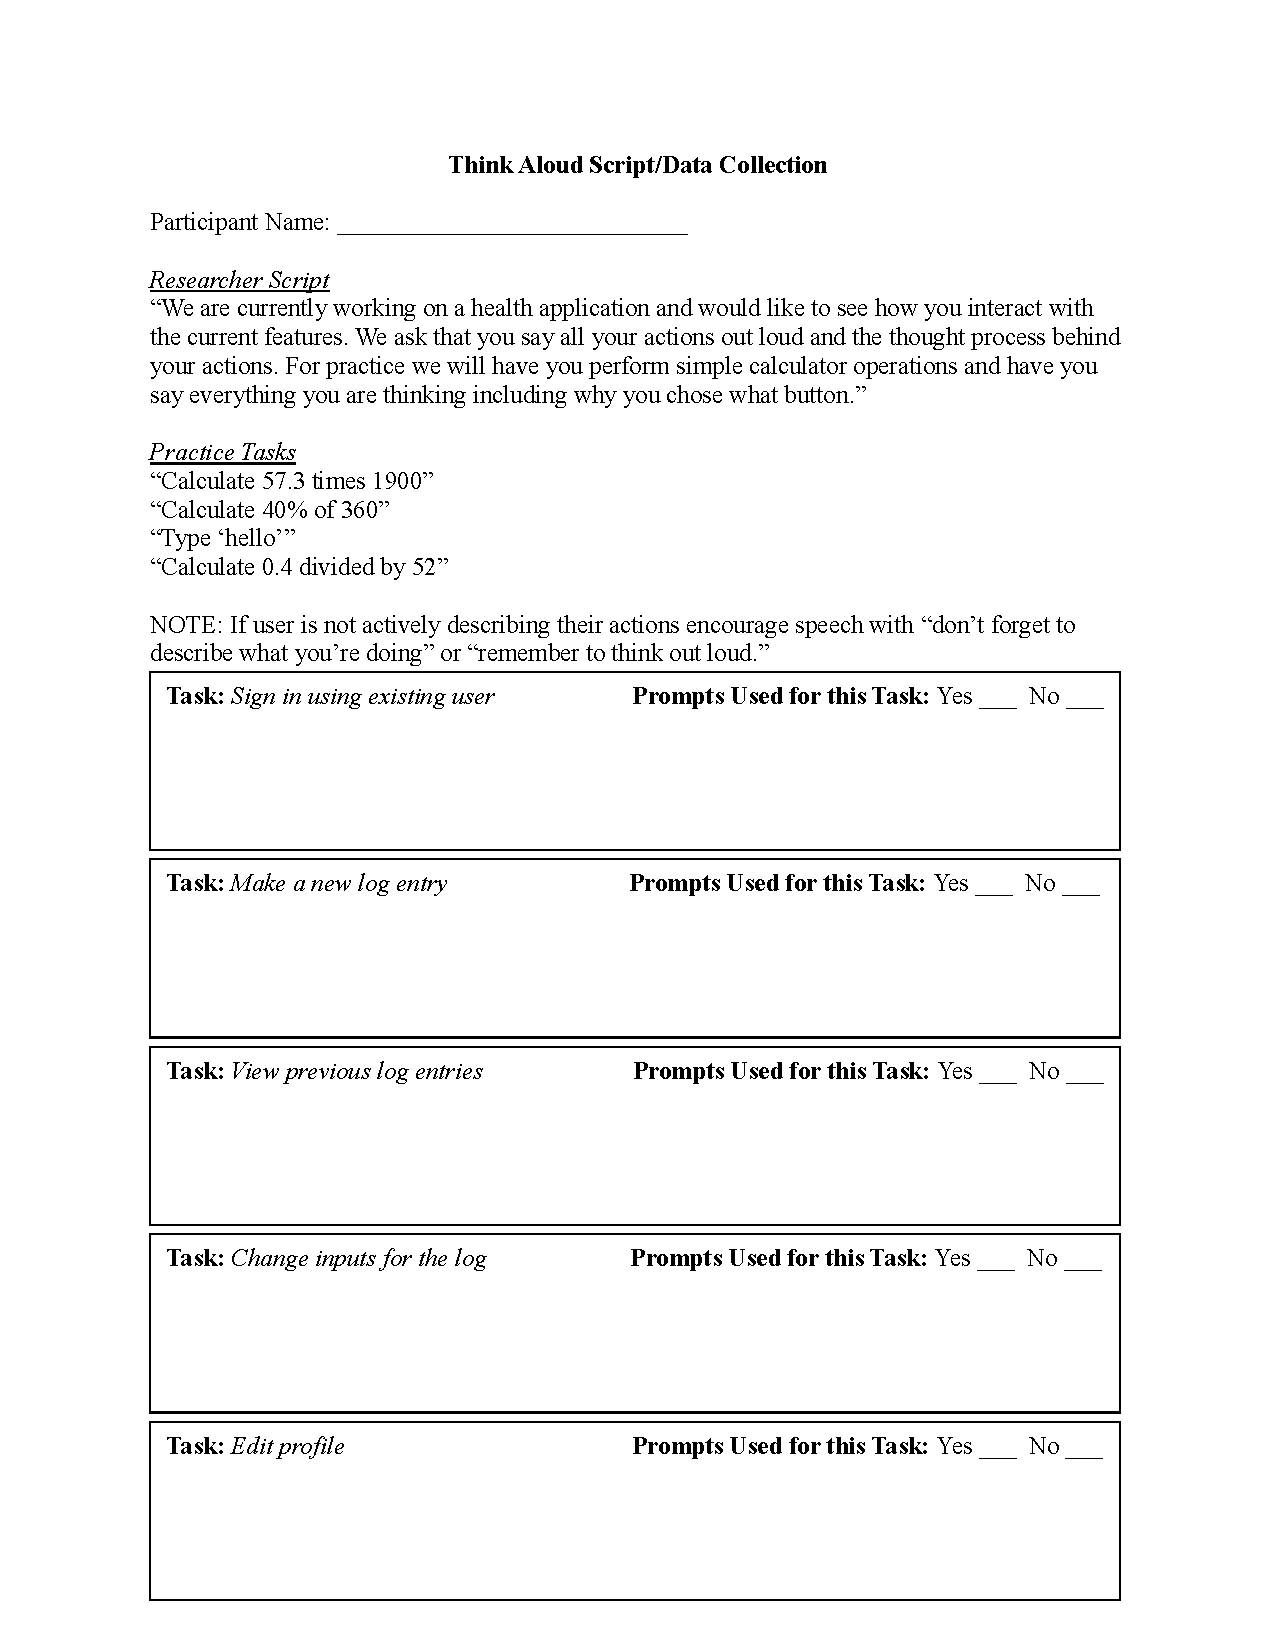
\includepdf[pages=-]{Screens/ThinkAloudScript.pdf}

\section{Rationale}
Performing a think aloud is suitable for our application's current state since it allows us to gather data without needing any additional equipment; only the paper prototype and a participant is required. Also, since this method is quick and easy to perform, we are able to gather numerous participants and keep explanation of the task at hand to a minimum.
\section{Tasks}
\begin{itemize}
\item Sign in using existing user
\item Make a new log entry
\item View previous log entries
\item Change inputs for the log
\item Edit profile
\end{itemize}
\section{Participants}
The participants gathered for the think aloud varied in age: three of the five participants were aged 20-25 and the remaining two were between 40 and 45. The evaluators between the ages of 20 and 25 are currently attending post-secondary institutions while the remaining evaluators are currently working full time. All participants do own and operate smart phones, but only do so for their basic features. This implies that the users know basic smart phone maneuvering, but are not ``experts'' in any one task. None of the participants were previously exposed to the application in any form and will be seeing it for the first time while doing the think aloud
\chapter{Results}
\section*{Heuristic Evaluation}
\begin{center}
	\begin{tabular}{|p{\textwidth}|}
	\hline
	\textbf{User}: Full-Timer\\
	\hline
	\textbf{Name}: The term \emph{Add New} is ambiguous\\
	\hline
	\textbf{Problem/Good Aspect}: Problem\\
	\hline
	\textbf{Evidence}:
	\begin{itemize}
	\item{User managed to log in correctly and without problem, but when presented with the home screen he hesitated to \emph{Add New} stating ``Add new what?''}
	\item{Eventually it was tapped (mostly out of the large prominent nature of the button) and it brought him to the correct screen}
	\end{itemize}\\
	\hline
	\textbf{Explanation}:\\
	The user was able to log into the home page of the screen but was hesitant in pressing \emph{Add New} as, to him, it wasn't clear where clicking that button would take him. However, since the button took up the majority of the screen, he clicked the button resulting in the correct action. Once in the screen, he seemed to be more comfortable with the controls as he was able to complete and submit an entry. The overall time it took to complete this task was very short (ie: under a minute), but there were unclear segments as indicated by the user.\\
	\hline
	\textbf{Severity or Benefit}:
	\begin{itemize}
	\item{Rating: 2, minor usability problem}
	\end{itemize}
	\textbf{Justification(Frequency, Impact, Persistence)}:
	\begin{itemize}
	\item{\textbf{Frequency}:} Low - Only new users will not know the meaning of \emph{Add New} until clicked
	\item{\textbf{Impact}:} Low - Confusing at first, but users can click the button with no consequence
	\item{\textbf{Persistence}:} Low - After clicking the icon once, users will associate the action with the button
	\end{itemize}
	\textbf{How these factors are weighted and why}:\\
	All categories are low because of the fact that users will quickly learn what Add New does and there is no harmful consequence in clicking the button to begin with. Because of this, the problem can be considered a minor usability problem.\\
	\hline
	\textbf{Possible solution and/or trade-offs}:\\
	Make the \emph{Add New} button less ambiguous by using more descriptive text.\\
	\hline
	\end{tabular}
\end{center}

\begin{center}
	\begin{tabular}{|p{\textwidth}|}
	\hline
	\textbf{User}: Seneca Student\\
	\hline
	\textbf{Name}: No navigation or entry issues\\
	\hline
	\textbf{Problem/Good Aspect}: Good\\
	\hline
	\textbf{Evidence}:
	\begin{itemize}
	\item{User had no problem at all navigating through the screens: all the buttons were clicked in the correct order and the subject even said ``This is the easiest game ever!'' pointing out the simplicity in the task.}
	\end{itemize}\\
	\hline
	\textbf{Explanation}:\\
	The user had no question or hesitation in maneuvering through the different screens. The prominent size of the \emph{Add New} button clearly helped in his navigation.\\
	\hline
	\textbf{Severity or Benefit}:
	\begin{itemize}
	\item{Rating: 0, not a usability problem}
	\end{itemize}
	\textbf{Justification(Frequency, Impact, Persistence)}:
	\begin{itemize}
	\item{\textbf{Frequency}:} None - There are no issues arising in this situation
	\item{\textbf{Impact}:} None - Since the user was no confronted with any problems, there is no problem impact
	\item{\textbf{Persistence}:} None - If the user can navigate through the menu on their first try, all subsequent entries will be even simpler
	\end{itemize}
	\textbf{How these factors are weighted and why}:\\
	There was no issue presented when this user was navigating through screens so it is not considered a usability problem.\\
	\hline
	\textbf{Possible solution and/or trade-offs}:\\
None needed\\
	\hline
	\end{tabular}
\end{center}

\begin{center}
	\begin{tabular}{|p{\textwidth}|}
	\hline
	\textbf{User}: UofT Student \#1\\
	\hline
	\textbf{Name}: The big plus sign is misleading and home screen should be different\\
	\hline
	\textbf{Problem/Good Aspect}: Problem\\
	\hline
	\textbf{Evidence}:
	\begin{itemize}
	\item{``What does the big plus sign mean? Is that where you would add a new custom category?''}
	\item{``Why wouldn't logging in bring me directly to the entry screen?''}
	\end{itemize}\\
	\hline
	\textbf{Explanation}:\\
	This user is more familiar with the goal and implementations of the app, but was confused as to why logging in wouldn't bring him to the entry screen. When confronted with the home screen, further confusion was met with the large plus sign on the \emph{Add New} button. The user clicked it in order to get to the correct screen, but there were questions as to why things were placed the way that they were.\\
	\hline
\textbf{Severity or Benefit}:
	\begin{itemize}
	\item{Rating: 2, minor usability problem}
	\end{itemize}
	\textbf{Justification(Frequency, Impact, Persistence)}:
	\begin{itemize}
	\item{\textbf{Frequency}:} Low - If the user has not seen the screen layout before, the icons and screen order will seem ambiguous, but only upon first use
	\item{\textbf{Impact}:} Low - Users can simply click the button to find out what it does with no consequence
	\item{\textbf{Persistence}:} Low - Once discovering what the button does, the user can become accustomed to the action and the screen order
	\end{itemize}
	\textbf{How these factors are weighted and why}:\\
	Again, all these categories are rated low because of the one-time occurrence of the problem and as such it is a minor usability problem.\\
	\hline
	\textbf{Possible solution and/or trade-offs}:
	\begin{itemize}
	\item{Make the \emph{Add New} button less ambiguous by using more descriptive text.}
	\item{Give the option to show the entry screen upon login as opposed to the given home screen}
	\end{itemize}\\
	\hline
	\end{tabular}
\end{center}
\begin{center}
	\begin{tabular}{|p{\textwidth}|}
	\hline
	\textbf{User}: Full-Timer\\
	\hline
	\textbf{Name}: Can't find the \emph{Settings} screen\\
	\hline
	\textbf{Problem/Good Aspect}: Problem\\
	\hline
	\textbf{Evidence}:
	\begin{itemize}
	\item{User went back and forth between screens the log entry screen and home screen before noticing the settings icon on the top right.}
	\item{Once in the \emph{Settings} screen, user scanned through the categories but did not know where he could add a custom category for the log entry.}
	\end{itemize}\\
	\hline
	\textbf{Explanation}:\\The user assumed that the settings for the log entries would be located in the log entry page, but could not find it. Instead of trying other options, the user went back and forth between the home page and the entry page hoping to see a clue that would lead him in the right direction. Eventually the icon was found on the home screen, but upon getting to the \emph{Settings} screen, the user did not know which category would complete the task because of the menu labeling.\\
	\hline
\textbf{Severity or Benefit}:
	\begin{itemize}
	\item{Rating: 3, major usability problem}
	\end{itemize}
	\textbf{Justification(Frequency, Impact, Persistence)}:
	\begin{itemize}
	\item{\textbf{Frequency}:} Moderate/High - This may occur every time the user wishes to change their entry settings
	\item{\textbf{Impact}:} High - The user was clearly confused in finding this setting and only overcame the issue once he scrutinized the screens. If the user wanted to do this quickly, he may end up giving up because of the complexity. 
	\item{\textbf{Persistence}:} Moderate - The user will get used to the settings menu over time, but because it is inconveniently placed, it is still a concern.
	\end{itemize}
	\textbf{How these factors are weighted and why}:\\
	Since customization is a key point in this application, the moderate/high frequency of this issue is followed by a high impact and moderate persistence leaving this to be a major usability problem.\\
	\hline
	\textbf{Possible solution and/or trade-offs}:\\
	Make the \emph{Settings} icon more prominent and available on every screen or give the user the direct ability to create a custom data field right from the log entry screen. This may reduce the minimalistic feel of the application, but it will increase it's convenience and functionality.\\
	\hline
	\end{tabular}
\end{center}

\begin{center}
	\begin{tabular}{|p{\textwidth}|}
	\hline
	\textbf{User}: Seneca Student\\
	\hline
	\textbf{Name}: Forgot task at hand because \emph{Settings} was too hard to find\\
	\hline
	\textbf{Problem/Good Aspect}: Problem\\
	\hline
	\textbf{Evidence}:
	\begin{itemize}
	\item{User logged in as normal, but immediately went into the \emph{Add New} section bringing up the log entry. He scrolled up and down trying to find a settings option and even attempted to find a pull down menu.}
	\item{After several attempts at finding \emph{Settings} he asked me ``What am I supposed to do again?'', in which I restated the task.}
	\item{Eventually I led him back to the \emph{Home Screen} and pointed out the icon on the top right hand corner and he exclaimed ``Oh, that's where it is.''}
	\end{itemize}\\
	\hline
	\textbf{Explanation}:\\The user went straight into the log entry screen and attempted to find settings from within that page. He tried numerous smartphone techniques such as long-tapping to bring up a sub-menu and swiping the top of the screen to bring down a drop-down menu (none of which were implemented in this app). The user went back and forth from the home screen to the entry screen and eventually forgot what his task was. I then pointed out where the \emph{Settings} icon was and relieved him from the rest of the task.\\
	\hline
\textbf{Severity or Benefit}:
	\begin{itemize}
	\item{Rating: 4, usability catastrophe}
	\end{itemize}
	\textbf{Justification(Frequency, Impact, Persistence)}:
	\begin{itemize}
	\item{\textbf{Frequency}:} Moderate/High - Users will want to customize the application as much as possible.
	\item{\textbf{Impact}:} High - The user could not find the \emph{Settings} menu at all leading them to forget about the task altogether
	\item{\textbf{Persistence}:} Moderate/High - Again, the user will eventually learn the nuances of the app over time, but because of the initial difficulty it may take a long time to overcome this issue
	\end{itemize}
	\textbf{How these factors are weighted and why}:\\
	Users will want to customize their app so that it suits their needs, thus having frequency heavily weighted. If the user is unable to find this feature, then it defeats the purpose of the application altogether placing this issue as a usability catastrophe.\\
	\hline
	\textbf{Possible solution and/or trade-offs}:\\
	Along with properly labeling the \emph{Settings} menu, give the option for sub-menus/settings within every screen either by long-tapping or special gestures. However, novice smartphone users may not discover these actions until frequent use of the application.\\
	\hline
	\end{tabular}
\end{center}

\begin{center}
	\begin{tabular}{|p{\textwidth}|}
	\hline
	\textbf{User}: UofT Student \#2\\
	\hline
	\textbf{Name}: Problematic labeling within \emph{Settings}\\
	\hline
	\textbf{Problem/Good Aspect}: Problem\\
	\hline
	\textbf{Evidence}:
	\begin{itemize}
	\item{User was able to find the \emph{Settings} icon quickly}
	\item{User clicked \emph{Medical History} first before clicking \emph{Change Log}, but was able to find the screen that would create a custom category.}
	\item{This user suggested that we call \emph{Change Log} ``Edit Categories'' instead}
	\end{itemize}\\
	\hline
	\textbf{Explanation}:\\This user has seen the screenshots before (during the CSC318 presentation) and was familiar with the different functions of the app. He had no trouble getting to the \emph{Settings} screen, but initially clicked \emph{Medical History} before \emph{Change Log}. Because of this error, he suggested that we call the category something more descriptive such as ``Edit Categories.''\\
	\hline
\textbf{Severity or Benefit}:
	\begin{itemize}
	\item{Rating: 2, minor usability problem}
	\end{itemize}
	\textbf{Justification(Frequency, Impact, Persistence)}:
	\begin{itemize}
	\item{\textbf{Frequency}:} Moderate/High - Users will want to utilize the customization feature very frequently
	\item{\textbf{Impact}:} Moderate - Not being able to quickly find this feature will limit the capability of the app greatly
	\item{\textbf{Persistence}:} Low - The user will quickly learn the functions of each category
	\end{itemize}
	\textbf{How these factors are weighted and why}:\\
	Since the user was able to overcome the issue quickly, the persistence of this issue for this user is low thus balancing the high frequency. This leads this issue to be a minor usability problem for this user.\\
	\hline
	\textbf{Possible solution and/or trade-offs}:\\
	Make the \emph{Change Log} setting less ambiguous by using more descriptive text.\\
	\hline
	\end{tabular}
\end{center}
\section*{Cognitive Evaluation}

\section*{Think-aloud Evaluation}
The results for the think aloud are compiled below. All tasks were performed in the order listed.
\begin{center}
	\begin{tabular}{|p{\textwidth}|}
	\hline
	\textbf{Sign in using existing user}\\
	\textbf{Note:} Users were told to assume that they knew the password if there is a password associated with the account\\
	\textbf{All users:} ``Open the app. Click the lock because that usually means enter a password. Enter the password and click okay.''\\
	\hline
	\textbf{Make a new log entry}\\
	\textbf{User 1 (20-25):} ``I'm going to assume that Add New refers to the new log entry so I will tap on that. Now I guess I'll change some values  in here and click OK!''\\
	\textbf{User 2 (20-25):} ``I'll click Add New. Now I'm going to change stuff in this screen.'' [Prompt user with ``Don't forget to say everything you're thinking''] ``Now I guess I have to save my choices. I'll click OK because that usually means save.''\\
	\textbf{User 4 (40-45):} ``There doesn't seem to be anything else to click except for the big plus sign so I'll choose that button. I don't know my blood sugar so I'll skip that part. What does Food(Image) mean? I guess I'll just click OK!''\\
	\hline
	\textbf{View previous log entries}\\
	\textbf{User 2 (20-25):} ``Click Previous Days because that should let me choose previous days. Now.. I think maybe just choose a day? [taps randomly]  Oh, I guess the green ones are days I can choose.''\\
	\textbf{User 3 (20-25):} ``I'm going to tap Previous Days because that's where I want to go. And from here I should pick a day that I want to view. Looks like the green ones are the ones I should pick from.''\\
	\textbf{User 5 (40-45):} ``The Previous Days button is pretty straightforward. Looks like the green buttons are clickable, but do I have to export something? Can I just click a specific day? [clicks on a day] Oh okay. I guess you just click the day.''\\
	\hline
	\textbf{Change inputs for the log}\\
	\textbf{User 1 (20-25):} ``So from the main screen I'll go into Add New maybe. [Scrolls back and forth] Doesn't really look like there's anything here, maybe go back to the main screen. Oh, is that a settings button in the corner? Okay from here I guess Change Log is the most logical place to go. And from here I can select what I want to include, right?''\\
	\textbf{User 4 (40-45):} ``I think that's a options button in the corner, I'm not sure, but let's see what it does anyway. Okay then from here I can click Change Log and it looks like these screens can change what you want to see.''\\
	\hline
	\textbf{Edit profile}\\
	\textbf{User 3 (20-25):} ``Editing profiles is usually done in a settings menu, so let's go there. So maybe from here I can just select my name or maybe Medical History depending on what you want to change.''\\
	\textbf{User 5 (40-45):} ``Where do you do that? The main screen? It doesn't look like there's anything there or in the entry screen. I guess it would have to be in that other screen from before (referring to the options screen). But it doesn't really look like you can change your info here, unless you meant to change my Medical History.''\\
	\hline
	\end{tabular}
\end{center}

\chapter{Discussion and Analysis}
Evaluation Criteria:
Consistency and Standards
Flexibility and Efficiency
Error Prevention
Visibility of System Status
Aesthetic and Minimal Design
\chapter{Implications}
\chapter{Design Improvement}
\chapter{Reflection}
\chapter{Appendix}
\section*{Screen Prototypes}

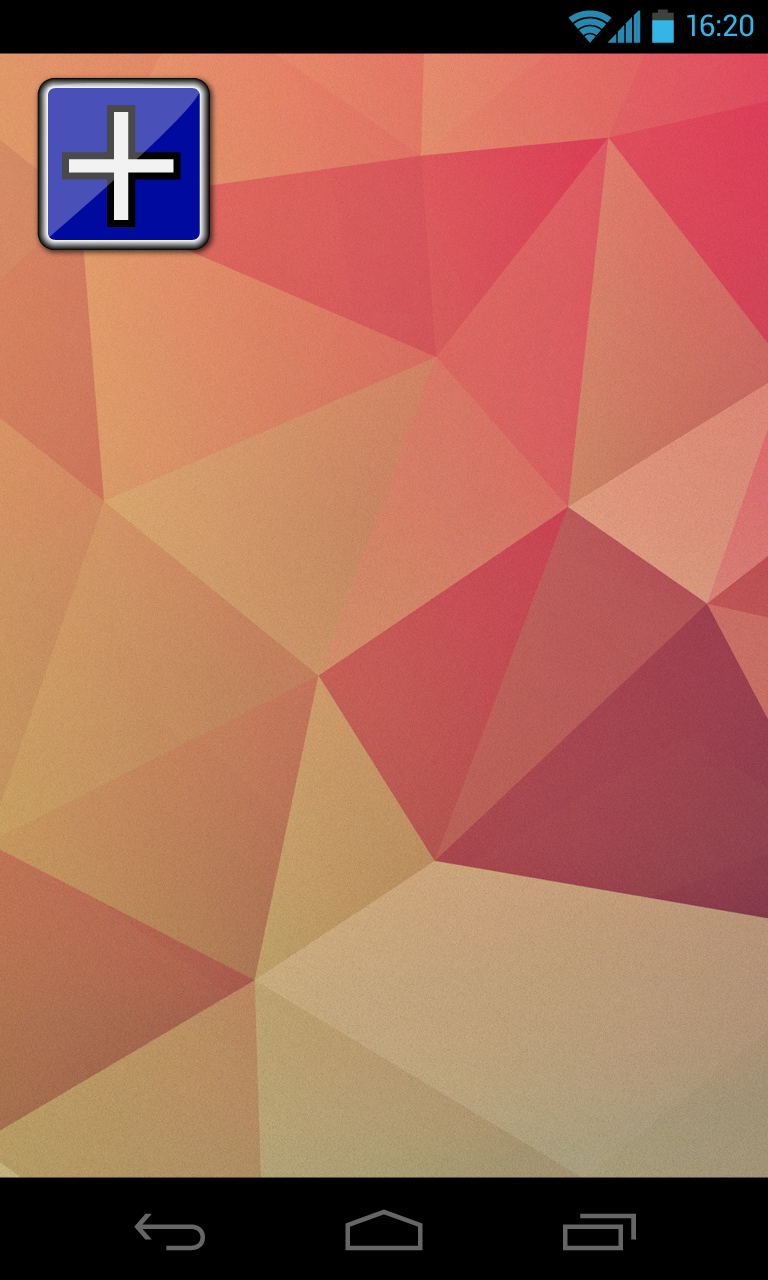
\includegraphics[scale=0.18]{Screens/00-Launch.png}
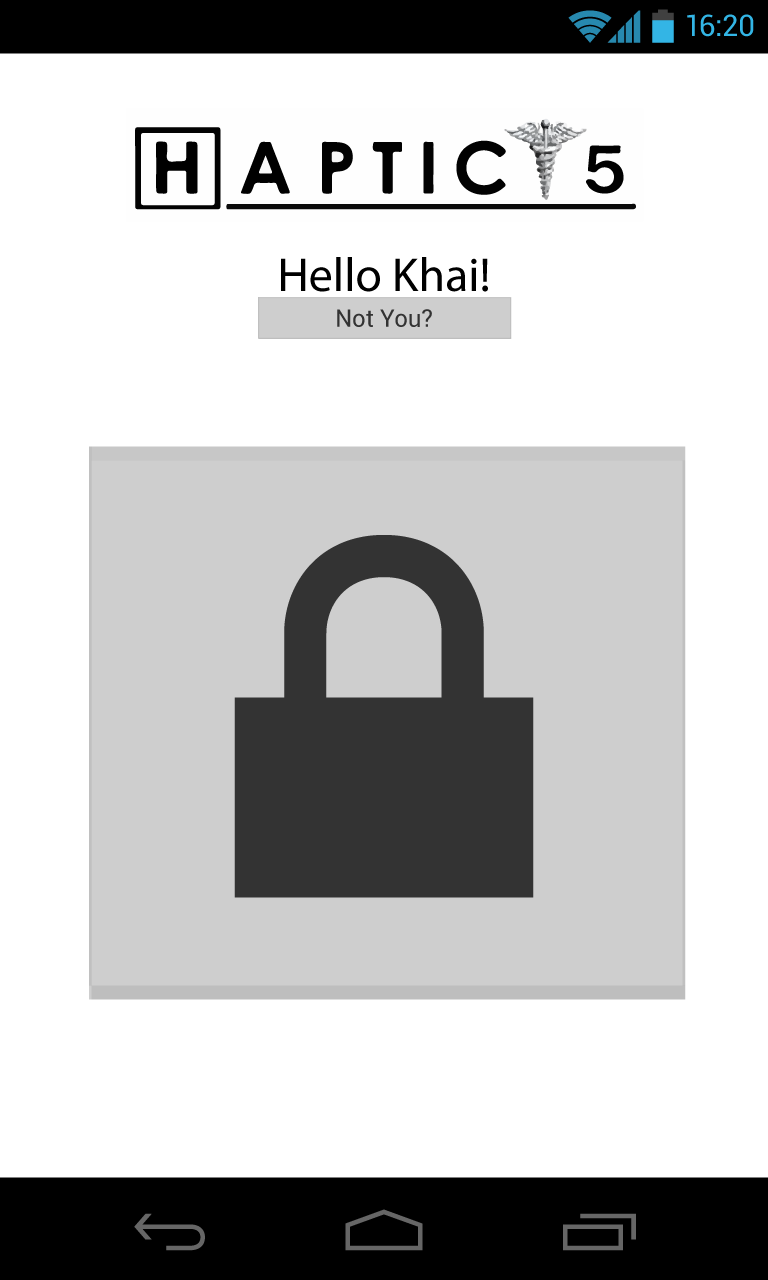
\includegraphics[scale=0.18]{Screens/00-Lock.png}
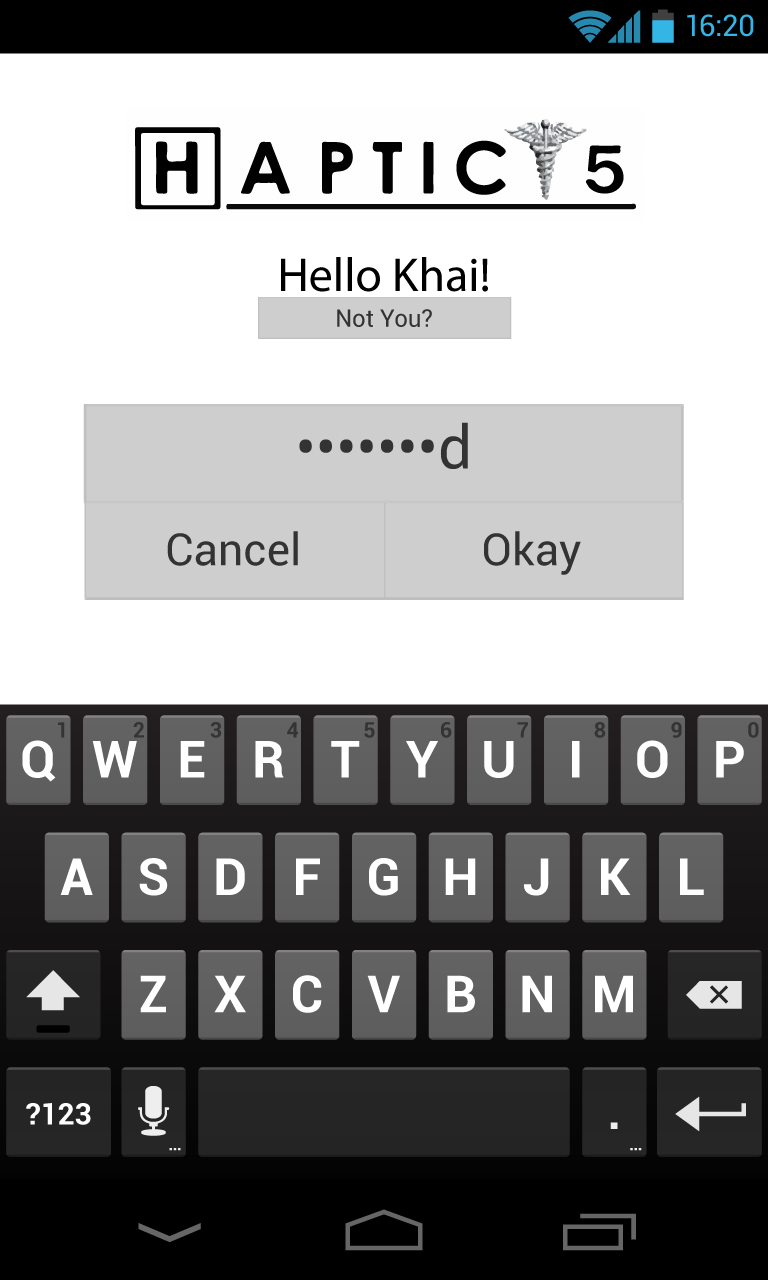
\includegraphics[scale=0.18]{Screens/00-Lock--Password-Entry.png}
\\\\
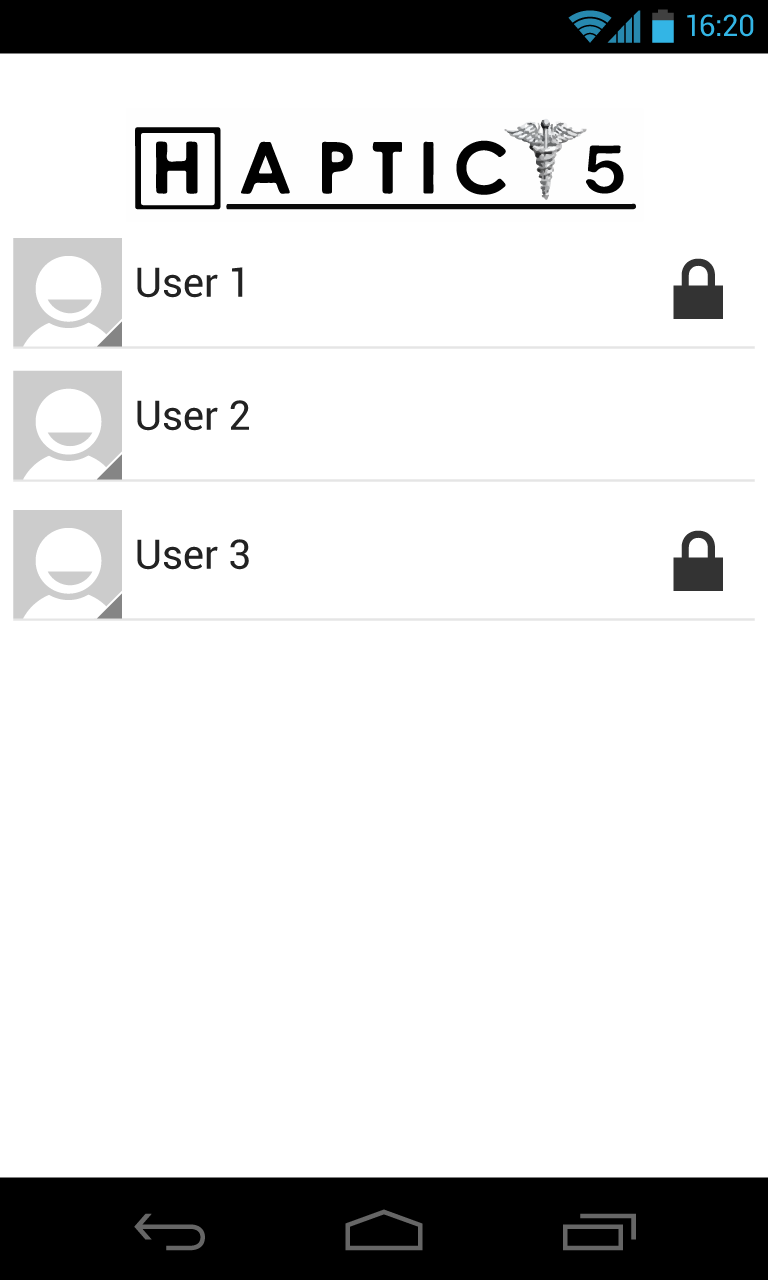
\includegraphics[scale=0.18]{Screens/01-Home---Change-User.png}
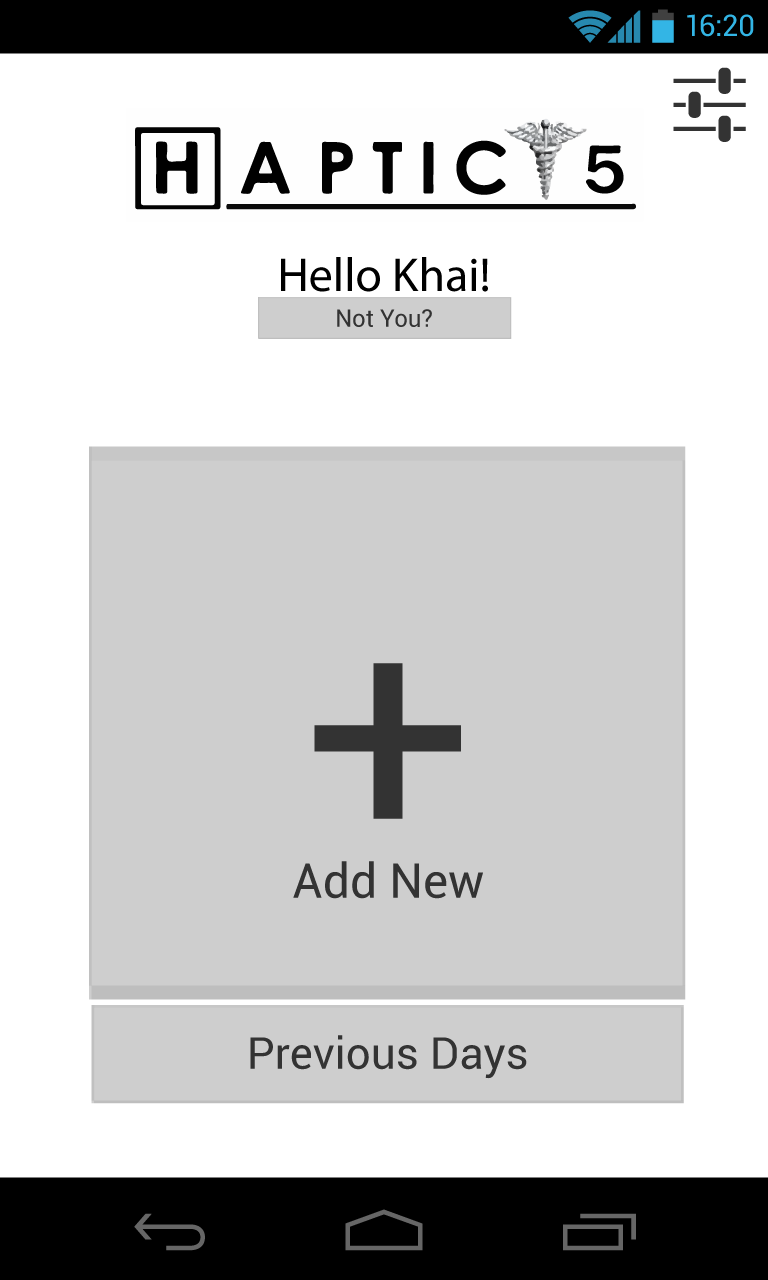
\includegraphics[scale=0.18]{Screens/01-Home---No-Selection.png}
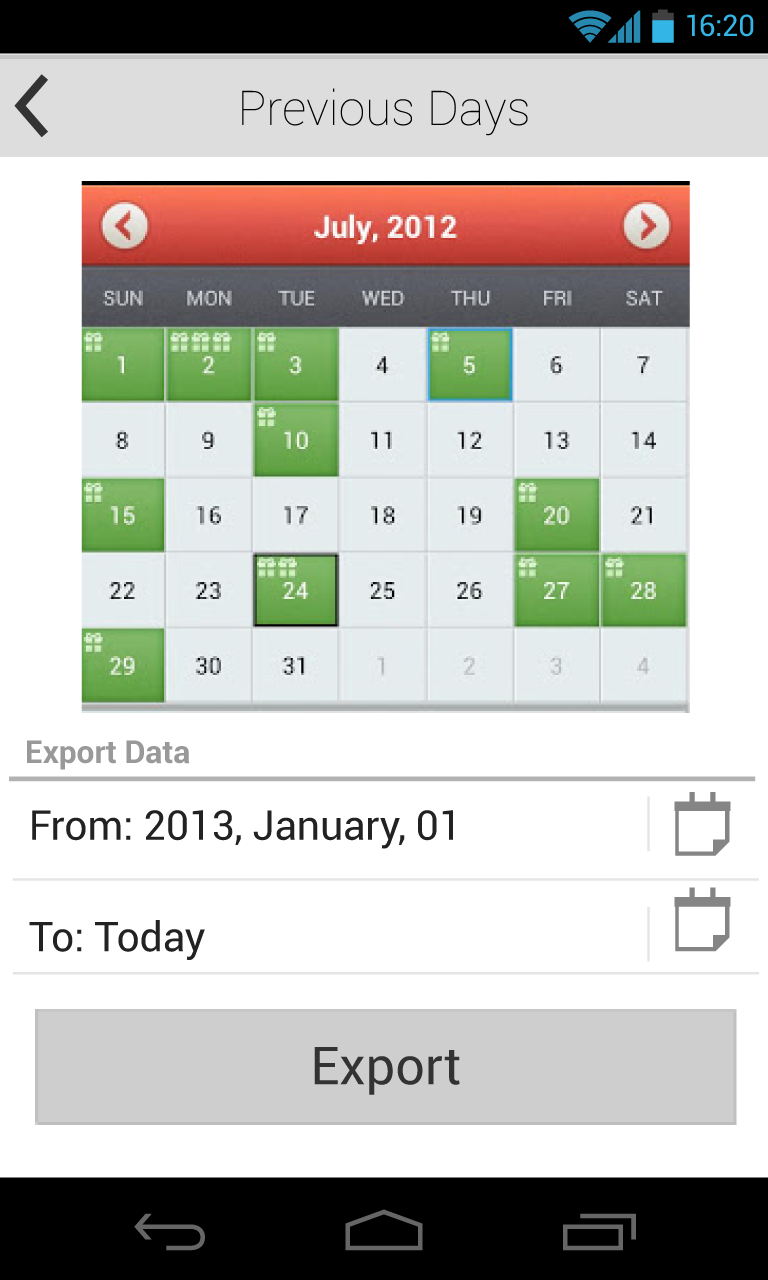
\includegraphics[scale=0.18]{Screens/02-Previous--No-Selection.png}
\\\\
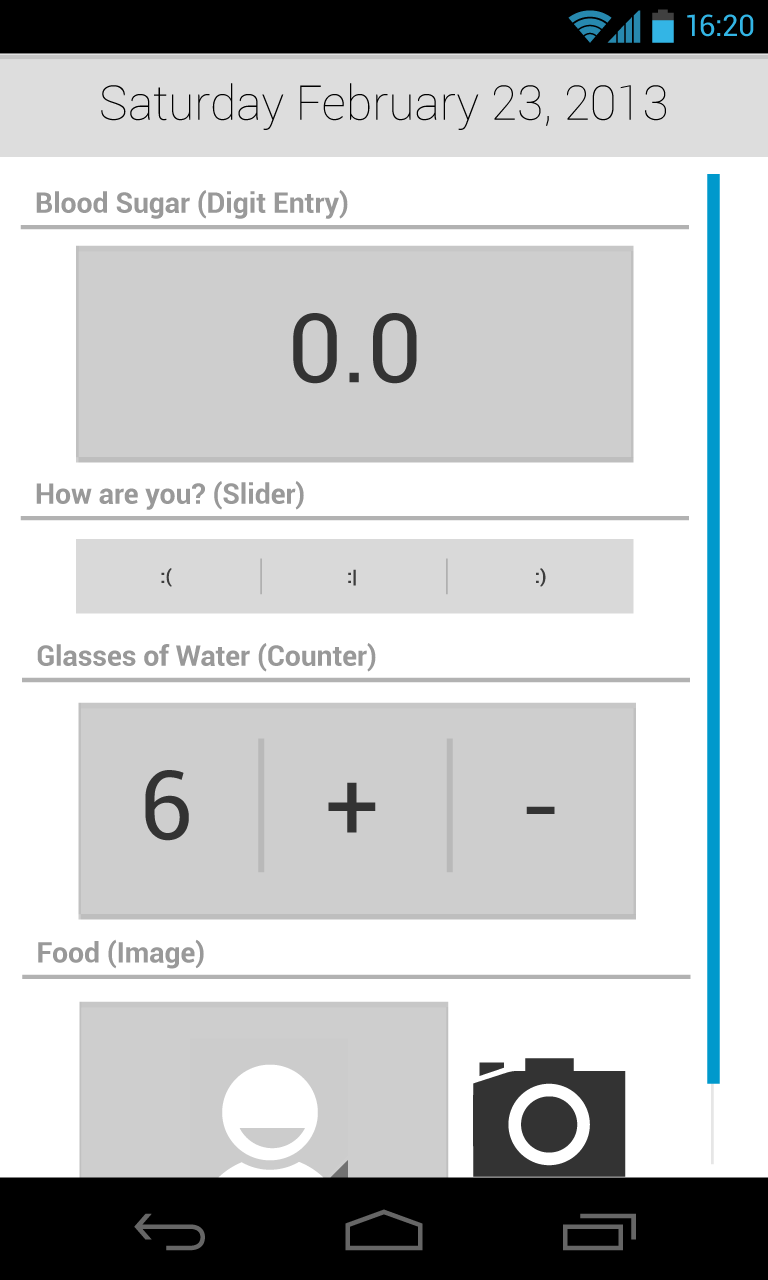
\includegraphics[scale=0.18]{Screens/03-Add--No-Selection.png}
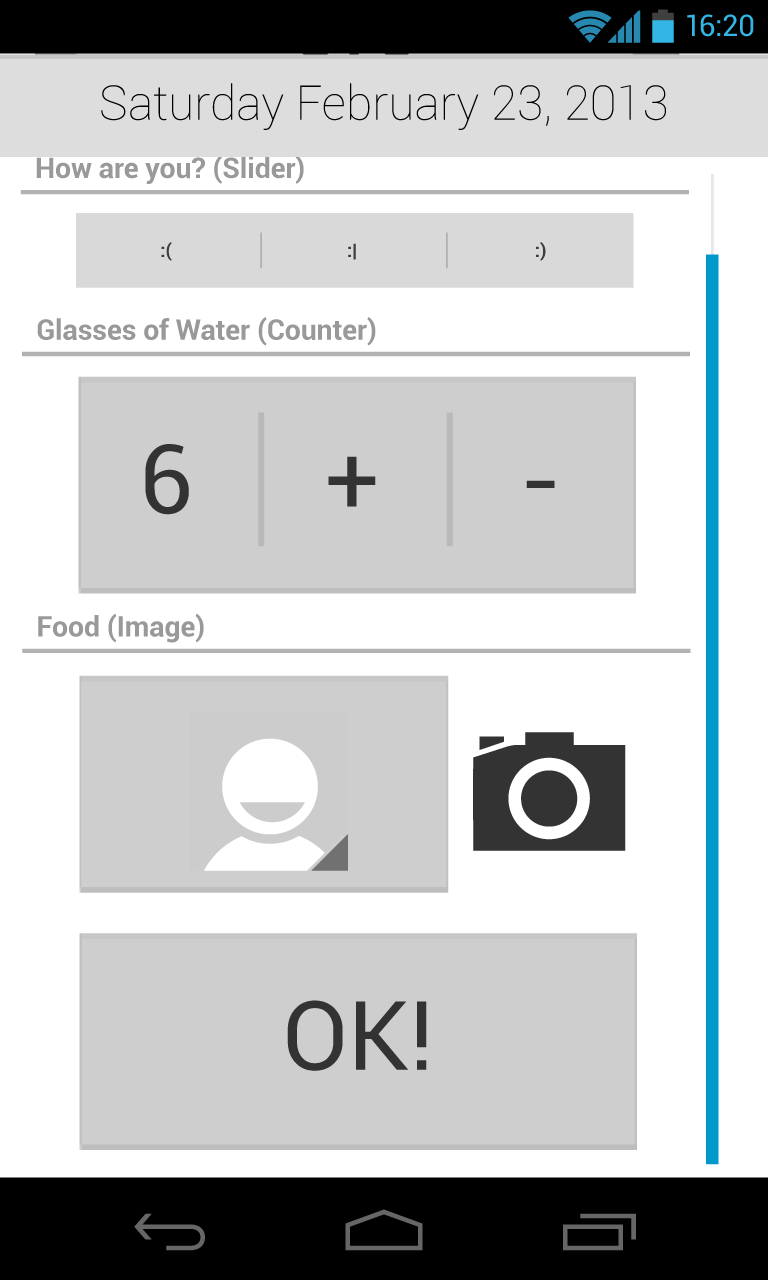
\includegraphics[scale=0.18]{Screens/03-Add--Scrolled.png}
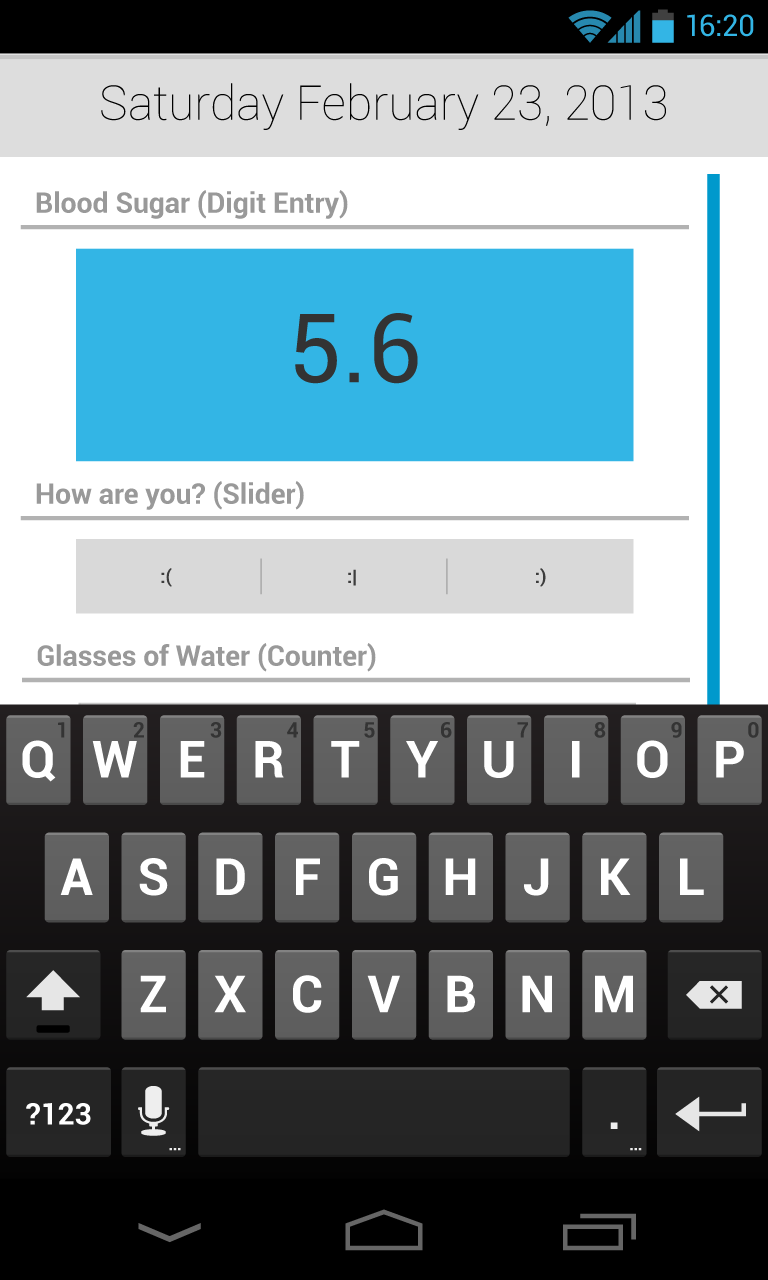
\includegraphics[scale=0.18]{Screens/03-Add--Add-Entry.png}
\\\\
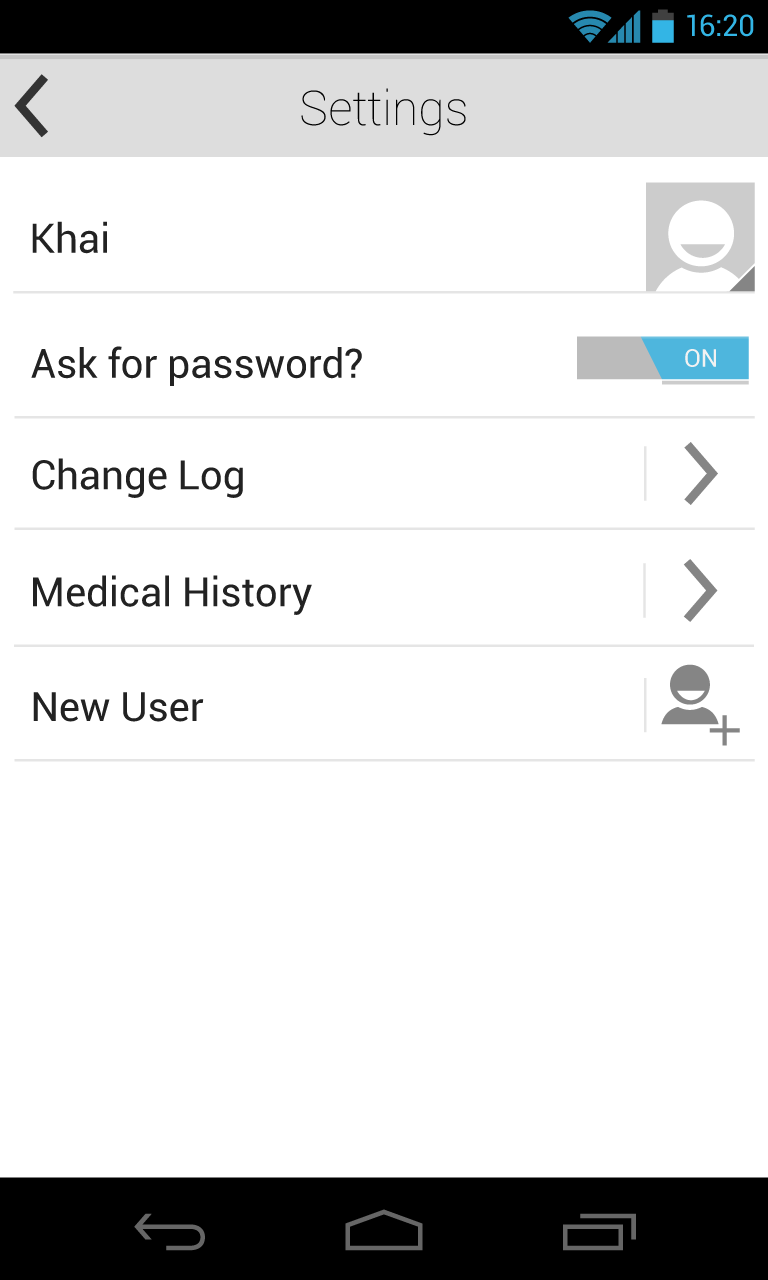
\includegraphics[scale=0.18]{Screens/04-Settings--Null.png}
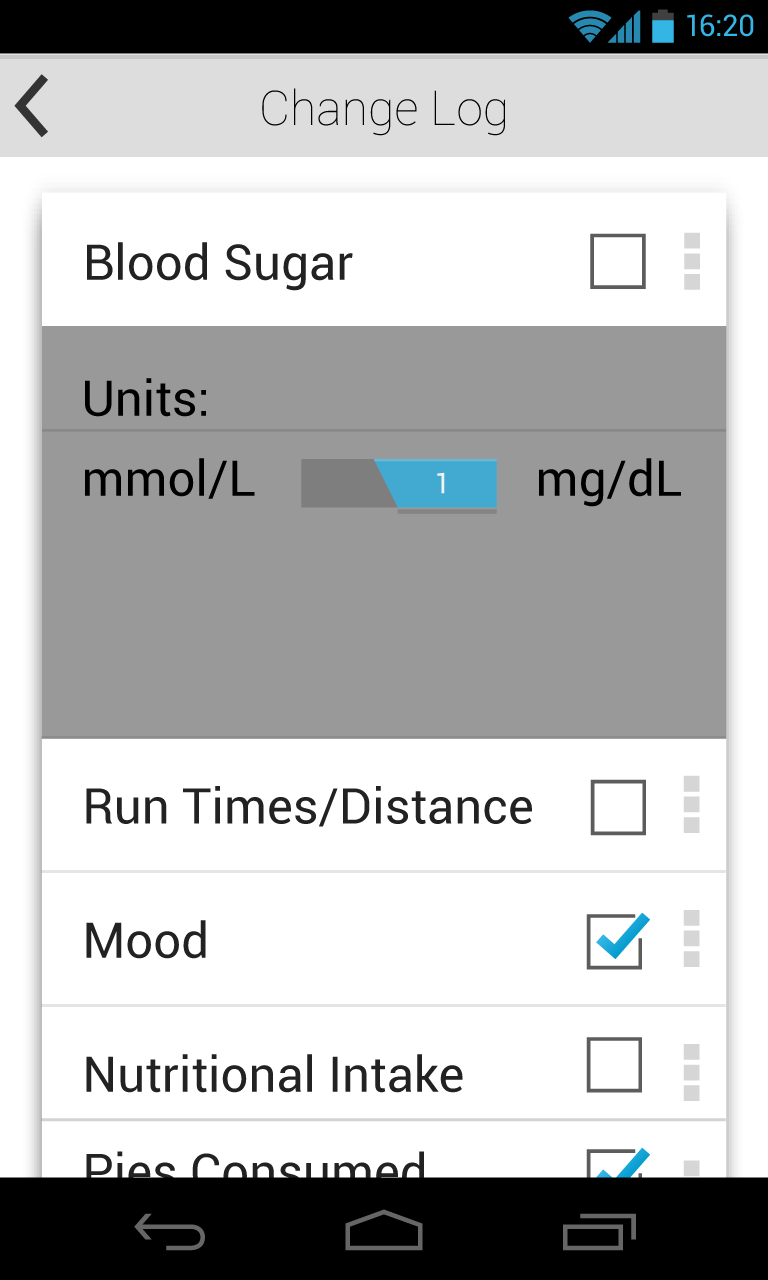
\includegraphics[scale=0.18]{Screens/05-Change-Log--Indi-Settings.png}
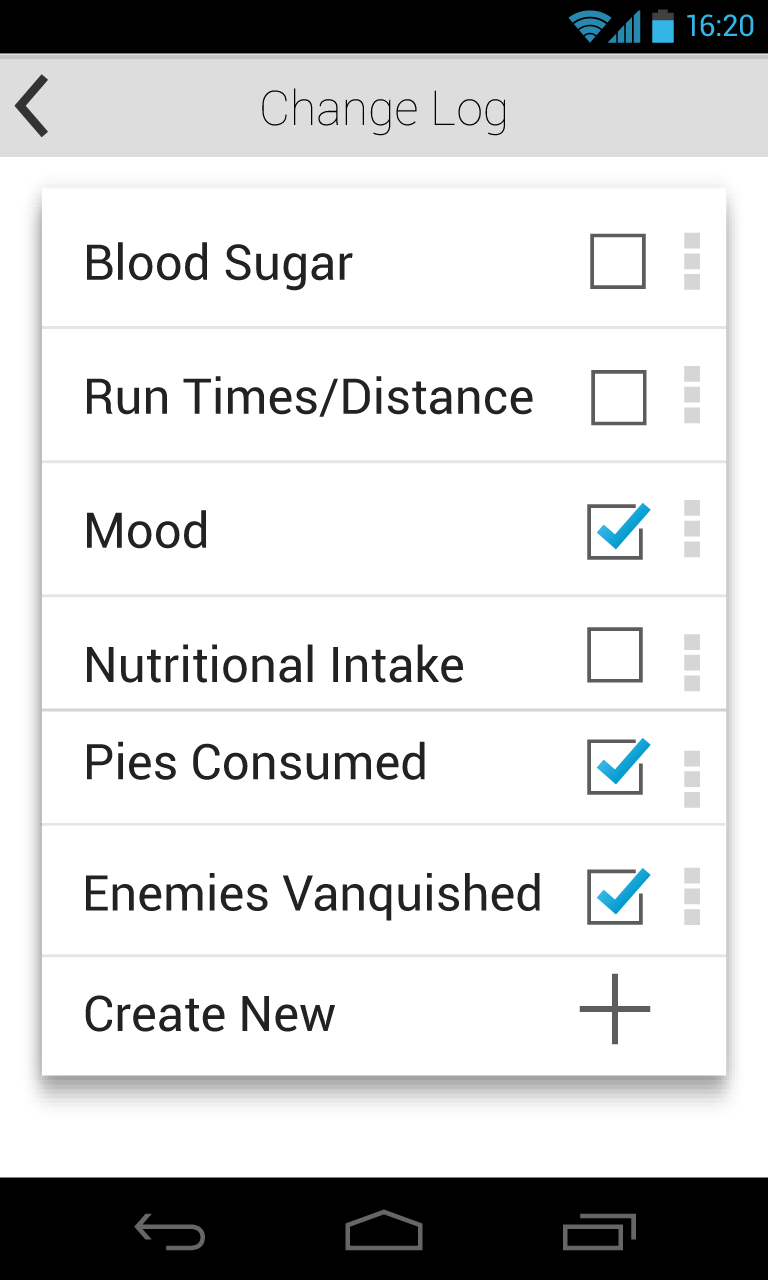
\includegraphics[scale=0.18]{Screens/05-Change-Log--Null.png}
\begin{enumerate}
\item{Phone Home Screen}
\item{Default User Screen (Password Protected)}
\item{Password Entry Screen}
\item{User Select Screen}
\item{User Home Screen}
\item{Previous Day Selection}
\item{Main Log Entry Screen}
\item{Main Log Entry Screen Scrolled Down}
\item{Selected Item Data Input}
\item{Settings Menu}
\item{Individual Category Customization}
\item{Category Menu}
\end{enumerate}
\section*{Sources}
http://www.cehd.umn.edu/nceo/OnlinePubs/Tech44/
\\http://www.nngroup.com/articles/thinking-aloud-the-1-usability-tool/




\end{document}
